\newif\ifdraft\draftfalse
\newif\ifjnf\jnffalse

\makeatletter \@input{texdirectives} \makeatother

\documentclass[10pt]{article}

\usepackage{fontspec}
\defaultfontfeatures{Ligatures=TeX}
\setmainfont{Palatino LT Std}
\setmonofont{Consolas}

\usepackage[margin=1in,includefoot]{geometry}

\usepackage{wrapfig}
\usepackage{graphicx}
\usepackage{xspace}

\newcommand{\petra}{Petr4\xspace}

\title{\bf Petr4: Formal Semantics for Programmable Networks}
\author{
Jialu Bao${}^*$~
Santiago Bautista${}^\dagger$~
Newton Ni${}^*$~
Rudy Peterson${}^*$~
Chris Sommers${}^\S$~
Nate Foster${}^*$~\\
$*$Cornell \quad $\dagger$ENS Rennes \quad $\S$Keysight
}

\begin{document}

\maketitle

\begin{wrapfigure}{r}{0.333\textwidth}
\vspace*{-1em}
\centerline{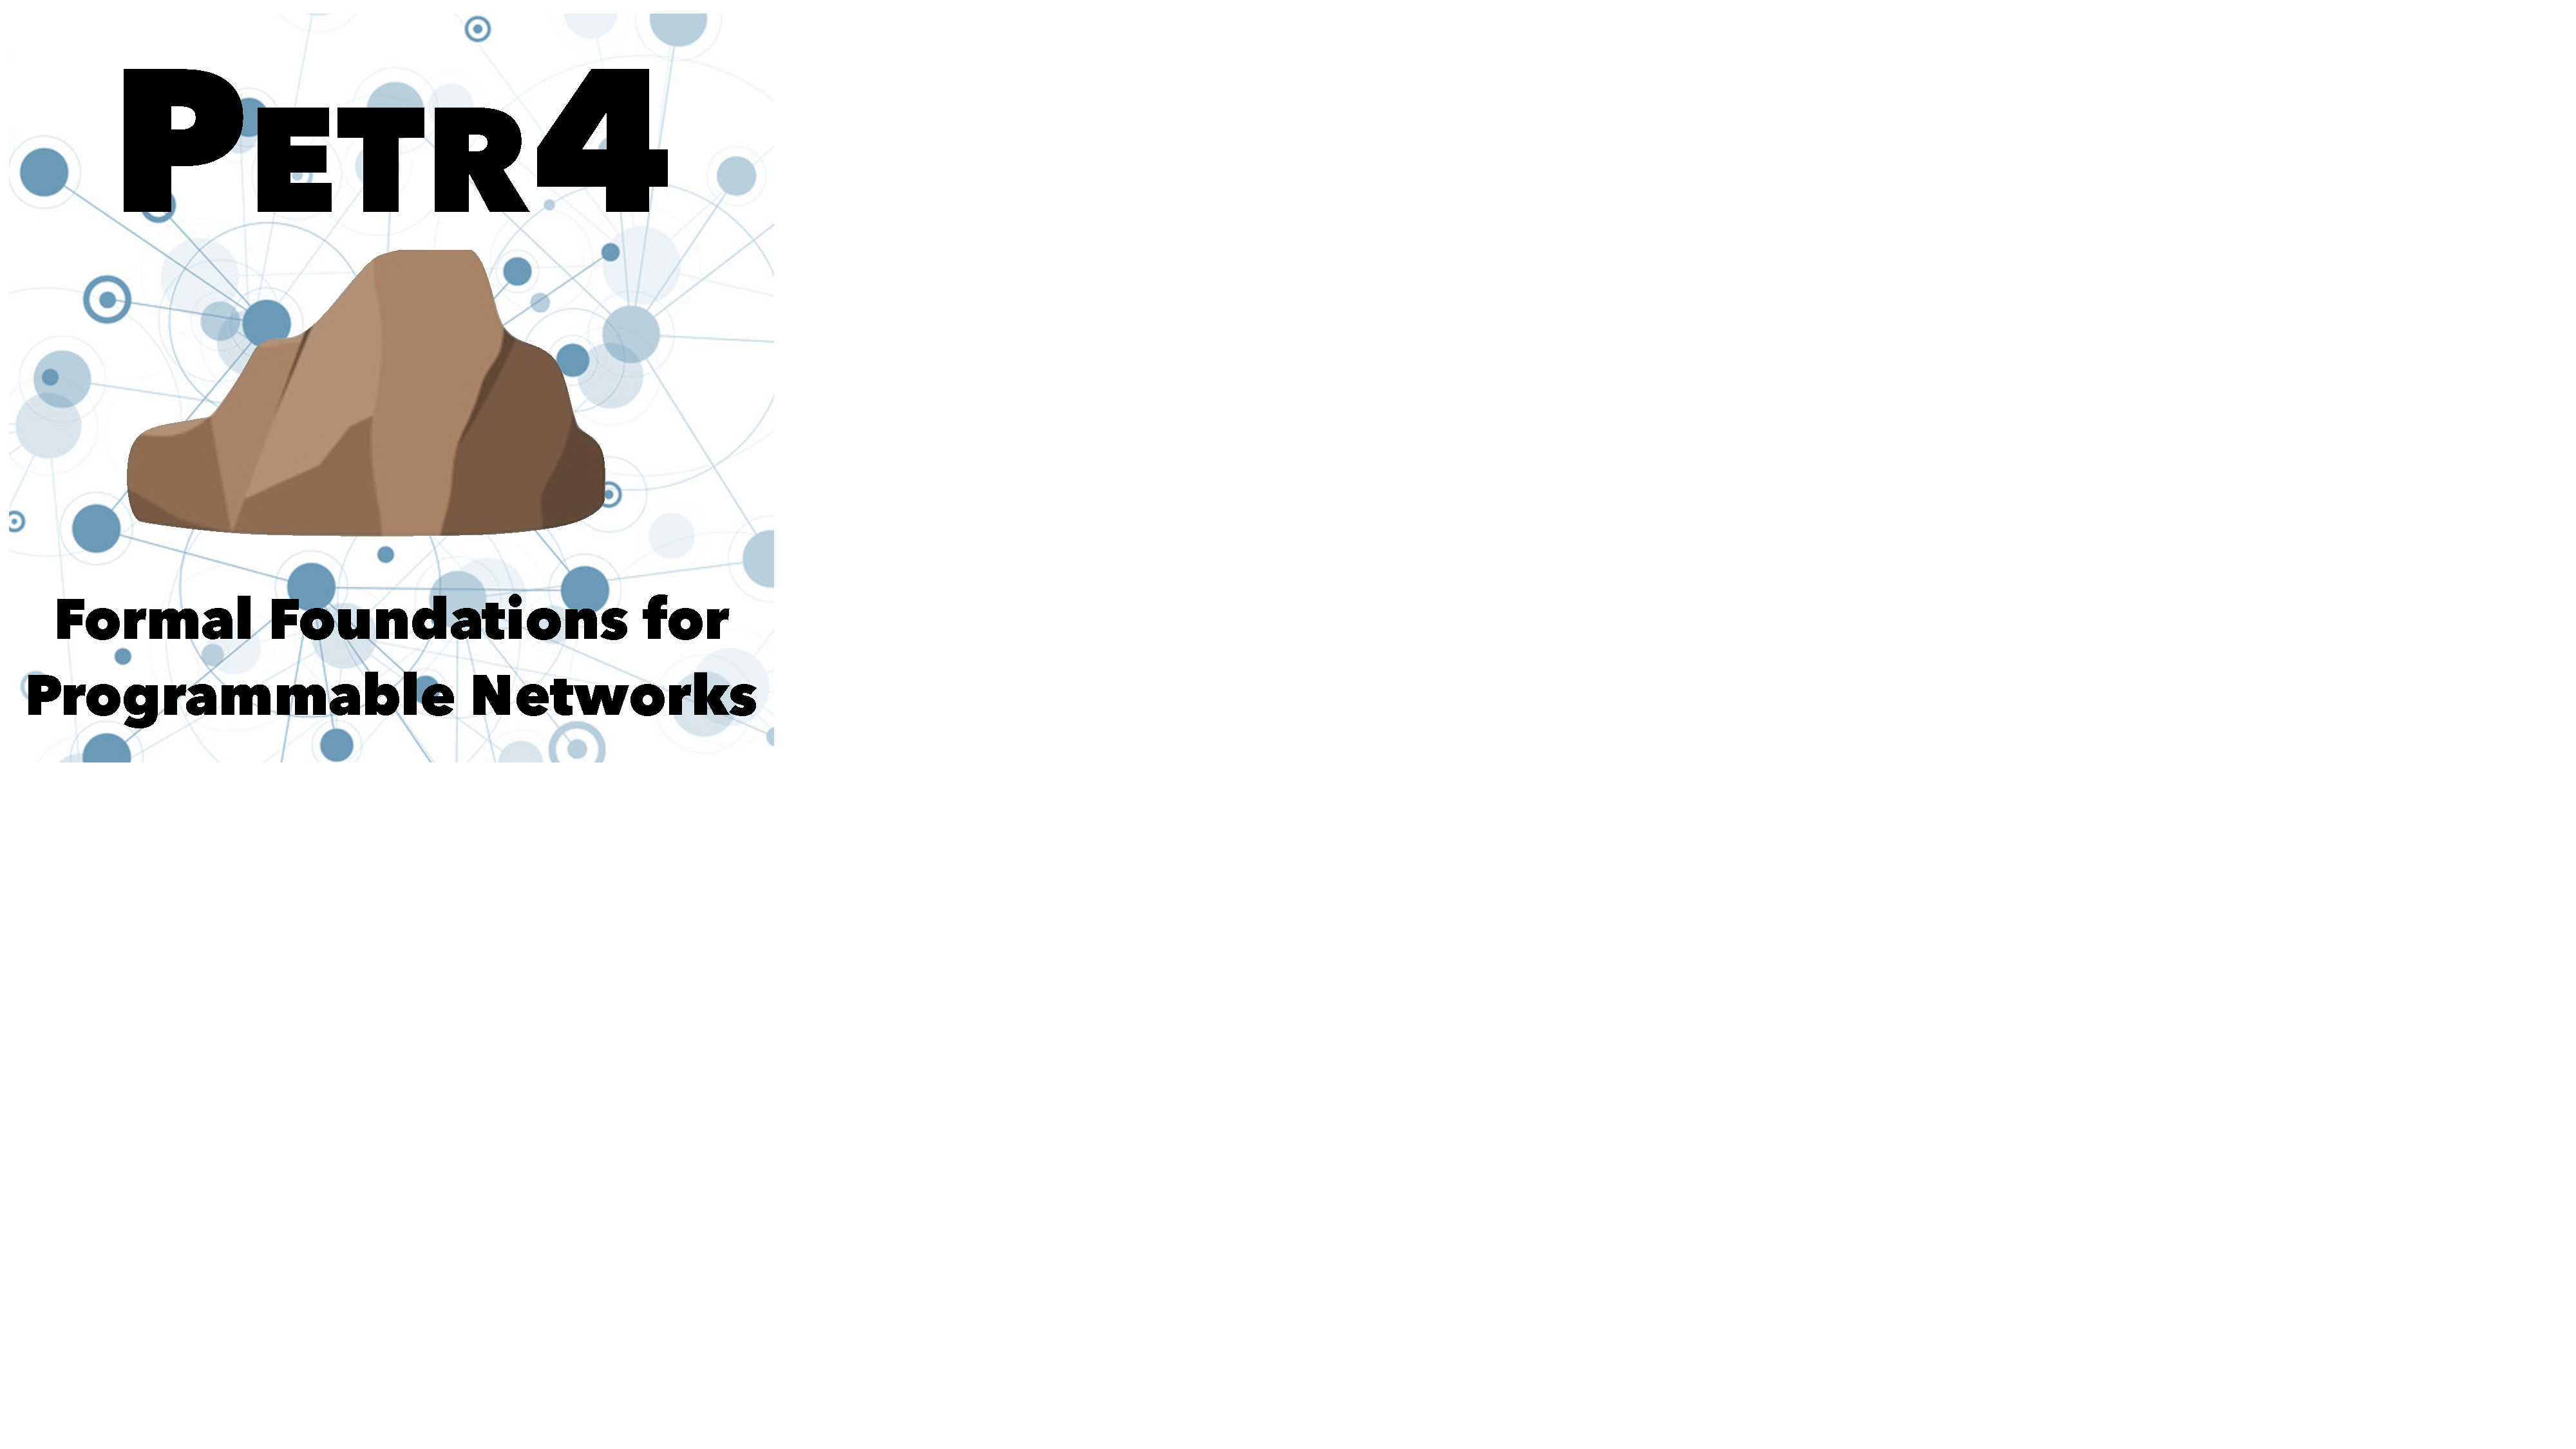
\includegraphics[width=0.3\textwidth]{logo}}
\end{wrapfigure}

The \petra project (pronounced ``petra'') is developing a new semantic
foundation for the P4 that clearly defines the behavior of every
language construct and assigns an unambiguous meaning to every
program. When completed, \petra will make it possible to apply a
variety of validation techniques to P4 data planes including
differential testing, fuzzing, symbolic execution, and deductive
verification.

Our work is inspired by recent successes in the formal methods
community, which have demonstrated that it is feasible to engineer
formal models of realistic software systems such as compilers,
distributed systems, and network controllers. We also leverage P4's
simplicity relative to general-purpose languages.

In preliminary work to date, we have developed an independent
front-end for P4$_{16}$ that handles all of the programs provided in
the test suite distributed with the open-source compiler. Because the
P4$_{16}$ grammar is ambiguous, we had to implement the ``lexer hack''
to distinguish between identifiers that represent variables and
identifiers that represent types. We discovered numerous
inconsistencies and typos in the language specification, as well as
bugs in the front-end of the open-source compiler. We are currently
working to formalize P4's type system and develop an
operational semantics. To achieve this, we are developing a core
language in which the higher-order programming constructs found in
P4$_{16}$ such as functions and object constructors have been
eliminated, and resources such as storage for headers and metadata
have been made explicit. For instance, while P4
has \texttt{switch} statements, \texttt{select} statements,
and \texttt{if}-\texttt{then}-\texttt{else} statements, the core
language might only support a single form of conditional.
To evaluate this semantics, we have built an OCaml implementation that
implements a reference interpreter.

In addition to formalizing the language, our work on \petra is also
informing language design. In particular, we are preparing a proposal
to extend P4$_{16}$ with new constructs for specifying the semantics
of architectures directly in the language. That is, the architecture
itself would provide a \texttt{main} function that describes the complete
sequence of P4 blocks it invokes to process packets. In support of
this goal, we imagine adding a new \texttt{fixed} construct to model
non-programmable elements such as the replication and queuing engine,
and a new \texttt{pipeline} construct to model compositions of parsers,
controls and fixed elements.

Although P4 is a relatively young language, there are already several
implementations, which sometimes make subtly different choices about
the meaning of programs. For example, if the \texttt{ingress} control
does not assign to the egress port, some targets drop the packet while
others forward it out port \texttt{0}. Having multiple diverse
implementations is healthy for the community, but also creates questions
about correctness.

To gain confidence in the fidelity of our formal semantics, we plan to
use differential testing to compare the results it computes against
all available open-source and commercial implementations. More
specifically, we plan to use a symbolic execution tool such
as \texttt{p4pktgen} to generate test packets with a high
degree of coverage. We will then develop a utility to compare test outputs,
ignoring non-deterministic factors---e.g., due to different choices made by
the scheduler. We will classify the discrepancies we discover and create
proposals for resolving any unintentional ambiguities found in the official
language specification.

\end{document}
